\documentclass[a4paper,11pt]{article}
\usepackage[colorlinks]{hyperref}
\usepackage{graphicx}
\usepackage{tikz-cd}
\usepackage{notestemplate}
\title{Motivic Homotopy Theory}
\author{Chow.}
\begin{document}
\maketitle
	\section{Construction of Unstable Homotopy Category}
	In order to refine the triangulated category of Voevodsky's motives and apply more tools from algebraic topology, we need well-behaved homotopy theory for schemes. Homotopy theory for schemes also allow us to construct motivic cohomology and algebraic K-theory which are looked as generalized cohomology theory defined with Brown representativity theorem.
	\subsection{Simplicial Sheaves and Hypercovers}
	Let us firstly recall some simplicial homotopy theory.
	$\Delta$ is category consists of objects such as
	\[
	[n]={0 \to 1 \to 2 \to \cdots \to n}
	\]
	for all non-negative integer $n$. And morphisms are functions of sets preserving the order of arrows.
	The category of \emph{simplicial sets} means the category of presheaves on $\Delta$ with values over $\mathbf{Sets}$. It is denoted by $\mathbf{sSets}$.
	
	In category of simplicial sets, we have following canonical objects
	\[
	\Delta[n] := \Delta(-,[n])
	\]
	They are call \emph{standard simplicial sets}.
	\begin{secprop}
		$\Delta([m],[n])$ is generated by following morphisms
		\[
		\begin{aligned}
			d^i \colon [k] &\to [k+1]\\
			d^i(0 \to 1 \to 2 \to \cdots \to k)&=\begin{cases}
			1\to 2 \to \cdots \to k+1& \text{if } i =0\\
			0 \to 1 \to \cdots \to i-1 \to i+1 \to \cdots \to k+1& \text{if } 1\leq i \leq k\\
			0 \to 1 \to \cdots \to k& \text{if } i =k+1\\
			\end{cases}
		\end{aligned} 
		\]
		and
		\[
		\begin{aligned}
		s^i \colon [k] &\to [k-1]\\
		s^i(0 \to 1 \to 2 \to \cdots \to k)&=\begin{cases}
		0\to 0 \to 1 \to \cdots \to k-1& \text{if } i =0\\
		0 \to \cdots \to i \to i  \to \cdots \to k-1& \text{if } 1\leq i \leq k-1\\
		\end{cases}
		\end{aligned} 
		\]
		where $d^i$ is called co-face map and $s^i$ is called co-degeneracy map.
	\end{secprop}
$\Delta$ is small category. As diagram, $\Delta$ looks like
\[
\begin{tikzcd} 
 {[0]} \arrow[r, shift left,"d^0"] \arrow[r, shift right,"d^1"'] & {[1]} \arrow[r,"d^0" description] \arrow[r, shift left=4,"d^1"] \arrow[r, shift right=4,"d^2"'] & \cdots 
\end{tikzcd}
\]
\[
\begin{tikzcd} 
{[0]} \arrow[r,"s^0",leftarrow] & {[1]} \arrow[r,shift left,"s^0",leftarrow] \arrow[r, shift right,"s^1"',leftarrow]  & \cdots 
\end{tikzcd}
\]
By Yoneda lemma, for simplicial set $X \in \mathbf{sSets}$, we have 
\[
X([n])\simeq \mathbf{sSets}(\Delta[n], X)
\]
\begin{figure}[h]
	\caption{Idea of simplicial sets (from nacatlab)}
\centering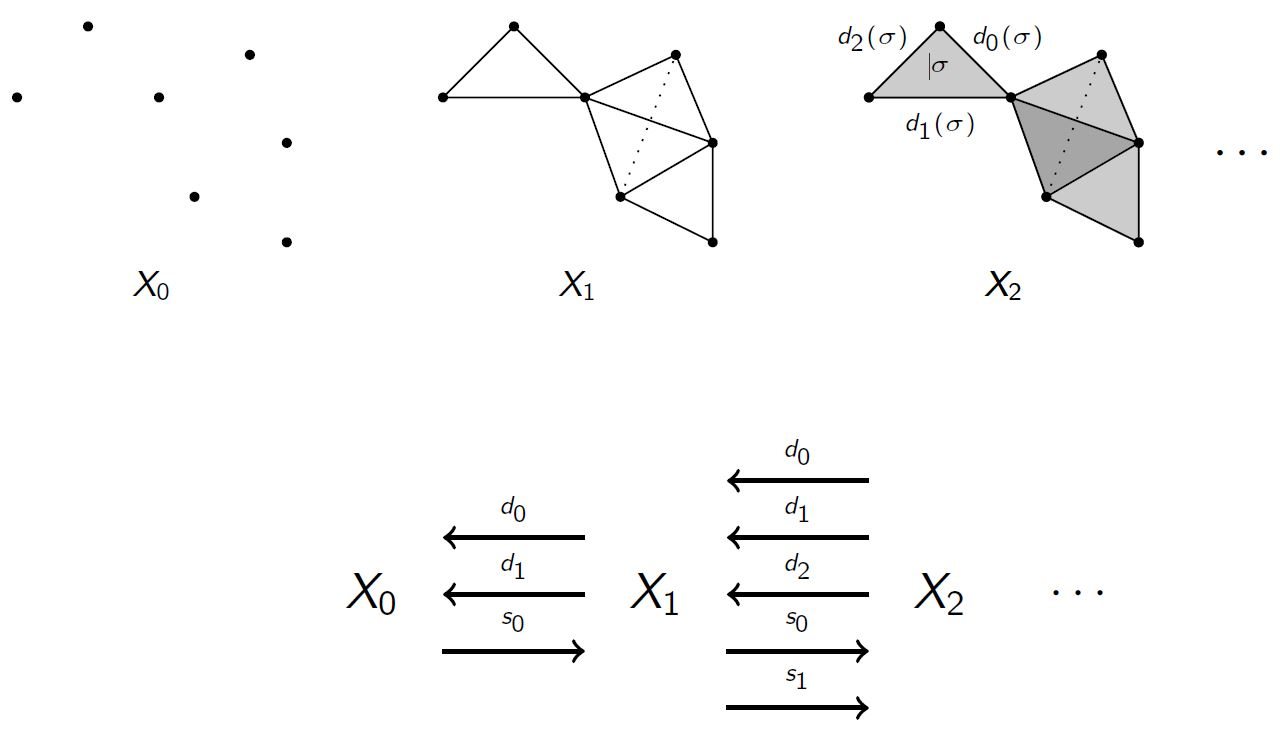
\includegraphics[scale=0.5]{PIC/SimplicialSetsIdea.jpg}
\end{figure}

In classical simplicial homotopy theory, we can endow $\mathbf{sSets}$ with model structure where fibrations are Kan fibrations and weak equivalence are morphisms which induce isomorphisms on homotopy groups.
\end{document}